% Created 2018-04-09 Mon 07:38
% Intended LaTeX compiler: pdflatex
\documentclass[10pt]{beamer}
\usepackage[utf8]{inputenc}
\usepackage[T1]{fontenc}
\usepackage{graphicx}
\usepackage{grffile}
\usepackage{longtable}
\usepackage{wrapfig}
\usepackage{rotating}
\usepackage[normalem]{ulem}
\usepackage{amsmath}
\usepackage{textcomp}
\usepackage{amssymb}
\usepackage{capt-of}
\usepackage{hyperref}
\usetheme{Boadilla}
\author{ECON 420: Game Theory}
\date{Spring 2018}
\title{Thinking about Games}
\usecolortheme{seagull}
\usefonttheme[onlylarge]{structurebold}
\usefonttheme[onlymath]{serif}
\setbeamerfont*{frametitle}{size=\normalsize,series=\bfseries}
\setbeamertemplate{navigation symbols}{}
\setbeamertemplate{itemize item}[triangle]
\setbeamertemplate{footline}{}
\setbeamertemplate{enumerate items}[default]
\hypersetup{
 pdfauthor={ECON 420: Game Theory},
 pdftitle={Thinking about Games},
 pdfkeywords={},
 pdfsubject={},
 pdfcreator={Emacs 25.2.2 (Org mode 9.1.6)}, 
 pdflang={English}}
\begin{document}

\maketitle

\begin{frame}[label={sec:org2405b21}]{}
\alert{Reading}
\begin{itemize}
\item This week: Chapters 1 and 2
\item Next week: Chapter 3
\end{itemize}
\end{frame}

\begin{frame}[label={sec:orgf243246}]{}
\alert{Nim}
\begin{itemize}
\item Today we'll play an alternative version of nim
\item One row of 20 lines
\item Each turn, the player must choose to remove 1, 2, or 3 lines
\item The last person to remove a line wins
\end{itemize}
$$|~|~|~|~|~|~|~|~|~|~|~|~|~|~|~|~|~|~|~|$$
\end{frame}

\begin{frame}[label={sec:org47ebe80}]{}
\begin{center}
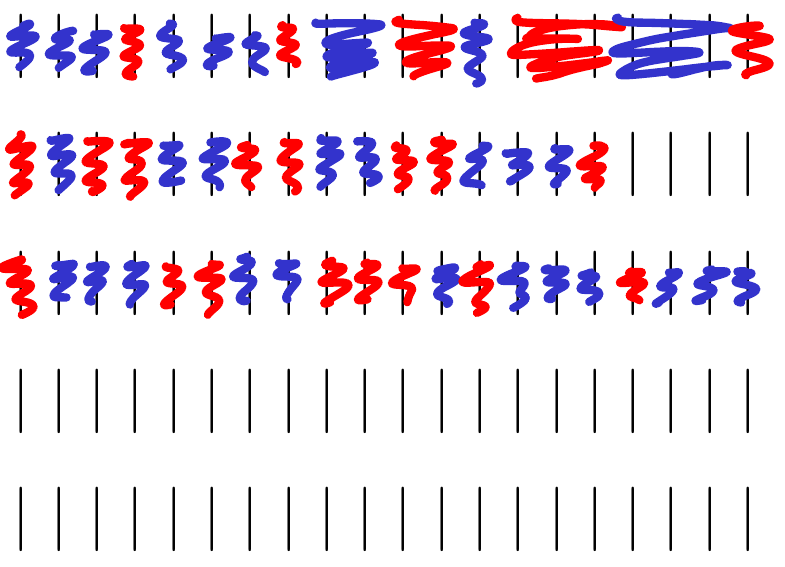
\includegraphics[width=.75\textwidth]{./img/nim.png}
\end{center}
\end{frame}

\begin{frame}[label={sec:org2b83ad3}]{}
\alert{Decisions vs games}
\begin{itemize}
\item \emph{Decisions} are choices that can be made "without concern for reaction or response from others"
\item \emph{Strategic games} (or just \emph{games}) are choices that occur among "mutually aware players"
\begin{itemize}
\item Players in strategic games take into account the cross-effects of their actions and the actions of other players
\end{itemize}
\end{itemize}
\end{frame}

\begin{frame}[label={sec:org400a9d2}]{}
\alert{Classifying games}
\begin{itemize}
\item Games can be:
\begin{itemize}
\item Sequential or simultaneous
\item Zero sum or non-zero sum
\item Single state or repeated
\begin{itemize}
\item Infinite or finite repetition
\end{itemize}
\item Perfect or imperfect information
\item Fixed or manipulable rules
\end{itemize}
\end{itemize}
\end{frame}

\begin{frame}[label={sec:org8ce3f9f}]{}
\alert{Sequential vs simultaneous games}
\begin{itemize}
\item Sequential games
\begin{itemize}
\item Players take turns (one after another)
\item Players look ahead at what might happen in the future to make choices
\end{itemize}
\item Simultaneous games
\begin{itemize}
\item Players make choices at the same time
\item Must predict what other players will do contemporaneously
\end{itemize}
\end{itemize}
\end{frame}

\begin{frame}[label={sec:orgf0c9512}]{}
\alert{Nim}
\begin{itemize}
\item Sequential or simultaneous?
\end{itemize}
\begin{itemize}
\item \emph{sequential}
\end{itemize}
\end{frame}

\begin{frame}[label={sec:orgbe93422}]{}
\alert{Rock, paper, scissors}
\begin{itemize}
\item Sequential or simultaneous?
\end{itemize}
\begin{itemize}
\item \emph{simultaneous}
\end{itemize}
\end{frame}

\begin{frame}[label={sec:org8305a0b}]{}
\alert{Chess}
\begin{itemize}
\item Sequential or simultaneous?
\end{itemize}
\begin{itemize}
\item \emph{sequential}
\end{itemize}
\end{frame}

\begin{frame}[label={sec:org594806d}]{}
\alert{A single play in American football}
\begin{itemize}
\item Sequential or simultaneous?
\end{itemize}
\begin{itemize}
\item \emph{simultaneous}
\end{itemize}
\end{frame}

\begin{frame}[label={sec:org777333b}]{}
\alert{A soccer penalty kick}
\begin{itemize}
\item Sequential or simultaneous?
\end{itemize}
\begin{itemize}
\item \emph{simultaneous}
\end{itemize}
\end{frame}

\begin{frame}[label={sec:org4ac8daa}]{}
\alert{Registering for classes}
\begin{itemize}
\item Sequential or simultaneous?
\end{itemize}
\begin{itemize}
\item ?
\end{itemize}
\end{frame}

\begin{frame}[label={sec:org20d997c}]{}
\alert{Constant-sum vs non-constant-sum games}
\begin{itemize}
\item Constant sum
\begin{itemize}
\item The sum total payoffs are fixed
\item Playing the game only determines the allocation of payoffs, not the total amount
\end{itemize}
\item Zero sum
\begin{itemize}
\item A special case of constant sum where total payoffs are zero
\item Often used to refer to constant-sum games
\end{itemize}
\item Non-constant sum
\begin{itemize}
\item Total payoffs depend on choices of players
\end{itemize}
\end{itemize}
\end{frame}

\begin{frame}[label={sec:orge6647b1}]{}
\alert{Nim}
\begin{itemize}
\item Constant or non-constant sum?
\end{itemize}
\begin{itemize}
\item \emph{constant (zero)}
\end{itemize}
\end{frame}

\begin{frame}[label={sec:org4d81059}]{}
\alert{Rock, paper, scissors}
\begin{itemize}
\item Constant or non-constant sum?
\end{itemize}
\begin{itemize}
\item \emph{constant (zero)}
\end{itemize}
\end{frame}

\begin{frame}[label={sec:org347e7bd}]{}
\alert{Splitting the last piece of cake with someone}
\begin{itemize}
\item Constant or non-constant sum?
\end{itemize}
\begin{itemize}
\item \emph{constant (not zero)}
\end{itemize}
\end{frame}

\begin{frame}[label={sec:org86c765e}]{}
\alert{Chicken (stay straight or swerve)}
\begin{itemize}
\item Constant or non-constant sum?
\end{itemize}
\begin{itemize}
\item \emph{non-constant}
\end{itemize}
\end{frame}

\begin{frame}[label={sec:org99550ff}]{}
\alert{International trade}
\begin{itemize}
\item Constant or non-constant sum?
\end{itemize}
\begin{itemize}
\item \emph{non-constant}
\end{itemize}
\end{frame}

\begin{frame}[label={sec:org79e1c9f}]{}
\alert{Example}
\begin{itemize}
\item All-pay auction
\begin{itemize}
\item You will bid to receive a \$5 bill
\item You have to pay me your highest bid \emph{regardless if you win or lose the auction}
\item Everyone who bids has to pay, but only one person will win the \$5
\end{itemize}
\end{itemize}
\end{frame}

\begin{frame}[label={sec:org30825c8}]{}
\alert{Constant-sum games}
\begin{itemize}
\item Constant-sum games can be either:
\begin{itemize}
\item Negative sum (war, household chores)
\item Zero sum (sports, games with a "winner" and "loser")
\item Positive sum (eating cake)
\end{itemize}
\item Non-constant-sum games can be any of the above, too
\begin{itemize}
\item Sometimes positive \emph{and} negative sums are possible in the same game (all-pay auction)
\end{itemize}
\end{itemize}
\end{frame}

\begin{frame}[label={sec:org6dcce7c}]{}
\alert{Single-stage and repeated games}
\begin{itemize}
\item Single-stage games are played (against some particular opponents) and never again
\item Repeated games are played over and over
\begin{itemize}
\item Can be finitely or infinitely repeated
\item Choices in one round (stage) might affect later rounds (and vice versa)
\end{itemize}
\end{itemize}
\end{frame}

\begin{frame}[label={sec:org623360e}]{}
\alert{Golden Balls (split or steal)}
\begin{itemize}
\item Single-stage or repeated?
\end{itemize}
\begin{itemize}
\item \emph{single-stage}
\end{itemize}
\end{frame}

\begin{frame}[label={sec:org3e26b44}]{}
\alert{"Battle of wits" (poison cups)}
\begin{itemize}
\item Single-stage or repeated?
\end{itemize}
\begin{itemize}
\item \emph{single-stage}
\end{itemize}
\end{frame}

\begin{frame}[label={sec:org34c4cb7}]{}
\alert{A baseball plate appearance (pitcher vs batter)}
\begin{itemize}
\item Single-stage or repeated?
\end{itemize}
\begin{itemize}
\item \emph{repeated}
\end{itemize}
\end{frame}

\begin{frame}[label={sec:org5b2cdf0}]{}
\alert{OPEC oil production}
\begin{itemize}
\item Single-stage or repeated?
\end{itemize}
\begin{itemize}
\item \emph{repeated}
\end{itemize}
\end{frame}

\begin{frame}[label={sec:orga606763}]{}
\alert{Perfect and imperfect information}
\begin{itemize}
\item Perfect information
\begin{itemize}
\item Players know exactly what choice are available to each player and what the payoffs will be (given choices)
\end{itemize}
\item Imperfect information
\begin{itemize}
\item Uncertainty over choices or payoffs (or both)
\item External uncertainty: "Nature" (the state of the world) changes choices or payoffs
\item Strategic uncertainty: Imperfect information about what other players are doing or have done in the past
\end{itemize}
\end{itemize}
\end{frame}

\begin{frame}[label={sec:org8154b02}]{}
\alert{Nim}
\begin{itemize}
\item Perfect or imperfect information?
\end{itemize}
\begin{itemize}
\item \emph{perfect information}
\end{itemize}
\end{frame}

\begin{frame}[label={sec:org79aff5f}]{}
\alert{Chess}
\begin{itemize}
\item Perfect or imperfect information?
\end{itemize}
\begin{itemize}
\item \emph{perfect information}
\end{itemize}
\end{frame}

\begin{frame}[label={sec:org02f0b6d}]{}
\alert{Vacation planning}
\begin{itemize}
\item Perfect of imperfect information?
\end{itemize}
\begin{itemize}
\item \emph{imperfect information (external uncertainty)}
\end{itemize}
\end{frame}

\begin{frame}[label={sec:org6ccca2b}]{}
\alert{Applying for jobs}
\begin{itemize}
\item Perfect of imperfect information?
\end{itemize}
\begin{itemize}
\item \emph{imperfect information (strategic uncertainty)}
\end{itemize}
\end{frame}

\begin{frame}[label={sec:org26f67ae}]{}
\alert{Poker}
\begin{itemize}
\item Perfect of imperfect information?
\end{itemize}
\begin{itemize}
\item \emph{imperfect information (strategic uncertainty)}
\end{itemize}
\end{frame}

\begin{frame}[label={sec:orgec936ec}]{}
\alert{Fixed and manipulable rules}
\begin{itemize}
\item Fixed rules can't be altered by players
\item The choices available to each player are constant and known
\end{itemize}
\end{frame}

\begin{frame}[label={sec:org17da2a0}]{}
\alert{Nim}
\begin{itemize}
\item Fixed or manipulable rules?
\end{itemize}
\begin{itemize}
\item \emph{fixed}
\end{itemize}
\end{frame}

\begin{frame}[label={sec:orgee935f3}]{}
\alert{Political campaigns}
\begin{itemize}
\item Fixed or manipulable rules?
\end{itemize}
\begin{itemize}
\item \emph{manipulable}
\end{itemize}
\end{frame}

\begin{frame}[label={sec:org71dddb6}]{}
\alert{Advertising}
\begin{itemize}
\item Fixed or manipulable rules?
\end{itemize}
\begin{itemize}
\item \emph{manipulable}
\end{itemize}
\end{frame}

\begin{frame}[label={sec:org0323301}]{}
\alert{Defining a game}
\begin{itemize}
\item A strategic game must contain three elements:
\begin{enumerate}
\item Players
\item Strategies
\item Payoffs
\end{enumerate}
\item We make various assumptions about these elements
\end{itemize}
\end{frame}

\begin{frame}[label={sec:org59abdbb}]{}
\alert{Players}
\begin{itemize}
\item The participants in the game who make choices
\item Humans, firms, "nature", etc
\item We assume players are \emph{rational}
\begin{itemize}
\item They can calculate outcomes from different strategies and will choose the optimum
\end{itemize}
\item We assume players have \emph{common knowledge of the rules}
\begin{itemize}
\item Rules are fixed \emph{at some level}
\begin{itemize}
\item Example: Releasing tax returns when running for president
\item Example: Battle of wits
\end{itemize}
\item Whether or not to follow rules is \emph{itself} part of a larger game
\end{itemize}
\end{itemize}
\end{frame}

\begin{frame}[label={sec:orga97e7ad}]{}
\alert{Example}
Who are the players in a game of poker?
\end{frame}

\begin{frame}[label={sec:org5096f7e}]{}
\alert{Strategies}
\begin{itemize}
\item The set of choices available to the player
\item A complete strategy is a "map" (set of instructions) on how to play a game given any possible set of choices from the other players
\item Strategies are collections of choices
\item A strategy is complete if you could give your instructions to someone else (or a machine) to do
\end{itemize}
\end{frame}

\begin{frame}[label={sec:org58d3b0c}]{}
\alert{Payoffs}
\begin{itemize}
\item The outcomes of the game
\item Can be profits, utility, money, wins and losses, etc
\item In this class we will assume that higher payoffs are more desirable
\item We will often need to calculate \emph{expected payoffs} if there is some randomness or uncertainty (imperfect information)
\begin{itemize}
\item For any possible outcome \(i\) with payoff \(\pi_i\), expected payoffs are \(\sum_i p_i \pi_i\), where \(p_i\) is the probability of \(i\) occurring
\end{itemize}
\end{itemize}
\end{frame}
\begin{frame}[label={sec:orgaabec53}]{}
\alert{Examples}
\begin{enumerate}
\item Suppose I flip a coin
\begin{itemize}
\item Heads: You get \$100
\item Tails: You lose \$50
\end{itemize}
\item Suppose I flip 2 coins:
\begin{itemize}
\item Heads/heads: You get \$100
\item Heads/tails: You get \$20
\item Tails/tails: You lose \$40
\end{itemize}
\end{enumerate}
\end{frame}

\begin{frame}[label={sec:org737c8b1}]{}
\alert{Equilibrium}
\begin{itemize}
\item The outcome where nobody can do better by \emph{unilaterally} changing their strategy
\item At equilibrium, nobody can say "I wish I had done that differently"
\item Equilibrium does \emph{not} mean that the outcome is optimal
\item We don't expect to always obtain an equilibrium
\item There is \emph{at least} one equilibrium in every game
\end{itemize}
\end{frame}

\begin{frame}[label={sec:org221de48}]{}
\alert{One half the average game}
What is an equilibrium of this game?
\begin{itemize}
\item Everyone picks 0
\end{itemize}
\end{frame}

\begin{frame}[label={sec:orgc68fd2a}]{}
\alert{Extra-credit game (choosing points)}
What is an equilibrium of this game?
\begin{itemize}
\item Everyone chooses 1 point
\item Any other equilibria?
\end{itemize}
\end{frame}

\begin{frame}[label={sec:org4c65cb1}]{}
\alert{Guess the average}
\begin{itemize}
\item Everyone write down a number between 0 and 100
\item The winning number is the average number guessed
\item Trade papers after writing down your number
\end{itemize}
\end{frame}
\end{document}